\chapter{\uppercase{NCTM Case Study}}
The National Center for Therapeutic Medicine (NCTM) was used as a test bed for the original methodology. NCTM is a building located on the campus of Texas A\&M University, in College Station, Texas. 

The National Center for Therapeutics Manufacturing (NCTM) combines the educational and manufacturing focuses of the biopharmaceutical industry. The NCTM building is approximately 150,000 ft\textsuperscript{2} with nearly 50,000 ft\textsuperscript{2} of educational facilities that include wet labs, culture facilities, large lecture halls, and a mock current Good Manufacturing Practice (cGMP) training suite. Around 120,000 ft\textsuperscript{2} is on the first level and 30,000 ft\textsuperscript{2} is on the second level. 

The cGMP Suite contains modern biopharmaceutical manufacturing equipment that students can use to learn industry practices. The wet labs are equipped with chemical fume hoods and the necessary electronic equipment for following standard operating procedures used in the biopharmaceutical industry. The lecture halls seat up to 120 students and have large floor to ceiling windows. There is also an Apple Computer laboratory with 48 workstations on the second floor. 

On the academic side there are three dedicated outdoor air handling units that serve seven child air handling units. Two of the air handling units are constant speed and the others are variable air volume. OAHU 1-1 serves its own wet lab and also feeds into AHU 1-1 and AHU 1-2. OAHU 1-2 serves AHU 1-3 and 1-4 on the first floor. OAHU 2-1 serves three children air handlers on the second floor, AHU 2-1, 2-2, and 2-3. 

This document focuses on the academic side of the building since Utilities and Energy services with Texas A\&M University are only allowed to make immediate changes to the HVAC system on this side. In summary, the important parameters concerning NCTM are that it houses several biopharmaceutical labs, it has an academic side that can be immediately changed and a manufacturing side that cannot be immediately changed, and relies on dedicated outdoor air handling units to pretreat outdoor air. 

\begin{table}
\centering
\caption{Occupied/Unoccupied scheduling for the AHUs as described.}
\label{tab:OnOffSched}
\begin{tabular}{l c c c}
\toprule
Level 			& OAHU	 	& AHU \# 	& AHU Schedule 		 \\
\midrule
Floor 1 Area B	& OAHU 1-1  & N/A		& 24/7 	 \\
Floor 1 Area B 	& OAHU 1-1 	& AHU 1-1	& 24/7 	 \\
Floor 1 Area B 	& OAHU 1-1	& AHU 1-2	& 6am - 6pm, M-F 	 \\
Floor 1 Area A 	& OAHU 1-2 	& AHU 1-3	& 6am - 8pm, M-F	 \\
Floor 1 Area A 	& OAHU 1-2	& AHU 1-4	& 6am - 8pm, M-F 	 \\
Floor 2 		& OAHU 2-1	& AHU 2-1	& 6am - 10pm, M-F 	 \\
Floor 2 		& OAHU 2-1 	& AHU 2-2	& 6am - 10pm, M-F	 \\
Floor 2			& OAHU 2-1	& AHU 2-3	& 6am - 10pm, M-F 	 \\
\bottomrule
\end{tabular}
\end{table}

\begin{figure}
    \centering
\includegraphics[]{Plots/TempRiseVsFlow-AHU-2-14.pdf}
\caption{Temperature rise due to the mixing of plenum air at the terminal box for FPVAV-2-14. }
\end{figure}

\begin{table}
\caption{Fan schedule information for the dedicated outdoor air handlers.}
\label{tab:OAFanSched}
\centering
\begin{tabular}{l c c}
\toprule
OAHU & Design OA CFM & HP \\
\midrule
OAHU 1-1 & 12,800 & 20 \\
OAHU 1-2 & 4,500 & 5 \\
OAHU 2-1 & 2,200 & 2 \\
\bottomrule
\multicolumn{1}{r}{Total:} & 19,500 & 27 \\
\end{tabular}
\end{table}

\begin{table}
\centering
\caption{Fan schedule information for the AHUs.}
\label{tab:FanSched}
\begin{tabular}{l c c c c}
\toprule
AHU 	& Type	 	& Total Airflow (CFM) 	& HP 	& OA Served By\\
\midrule
AHU 1-1 & Constant  & 3,000 			  	& 5 	& OAHU 1-1 \\
AHU 1-2 & VAV 		& 4,800 				& 5 	& OAHU 1-1 \\
AHU 1-3 & VAV 		& 7,500 				& 7.5 	& OAHU 1-2 \\
AHU 1-4 & Constant 	& 5,000 				& 7.5 	& OAHU 1-2 \\
AHU 2-1 & VAV 		& 6,000 				& 7.5 	& OAHU 2-1 \\
AHU 2-2 & VAV		& 8.500					& 10 	& OAHU 2-1 \\
AHU 2-3 & VAV 		& 6,000					& 7.5	& OAHU 2-1 \\
\bottomrule
\multicolumn{2}{r}{Total:} & 40,800 & 50 &  \\
\end{tabular}
\end{table}

\section{Terminal Unit Information}

On the academic side, there are a total of 10 series fan powered terminal units on the first floor and 18 on the second floor. \tableref{} \ref{tab:TerminalUnitInformation} shows the design (and assumed constant) flowrates for each of the terminal units. 

\begin{table}[]
\centering
\footnotesize
\caption{Terminal unit information.}
\label{tab:TerminalUnitInformation}
\begin{tabular}{@{}llrl@{}}
\toprule
AHU &  Terminal Unit & \parbox{1.5cm}{Flow\\(CFM) }& Space Served \\ \midrule
%%\parbox{2cm}{AHU-1-1 \\ (5 hp)} & \multicolumn{3}{l}{No boxes - Serves Teaching Module alone, Constant Fan} \\ \midrule
AHU-1-2        & FPVAV-1-7 & 1,400 & Difficult to tell \\ \cmidrule(r){2-4}
(5 hp)         & FPVAV-1-8 & 700 & Vestible/Men's \& Women's bathroom \\  \cmidrule(r){2-4}
               & FPVAV-1-9 & 1,200 & Stairs/Front Corridor \\  \cmidrule(r){2-4}
               & FPVAV-1-10 & 1,600 & Hallway \\\midrule
AHU-1-3        & FPVAV-1-1 & 1,480 & Large Auditorium Lecture Hall \\  \cmidrule(r){2-4}
(7.5 hp)       & FPVAV-1-2 & 1,160 & Large Auditorium Lecture Hall \\  \cmidrule(r){2-4}
               & FPVAV-1-3 & 1,300 & Large Auditorium Lecture Hall \\  \cmidrule(r){2-4}
               & FPVAV-1-4 & 1,400 & Large Auditorium Lecture Hall \\  \cmidrule(r){2-4}
               & FPVAV-1-5 & 1,040 & Large Auditorium Lecture Hall \\  \cmidrule(r){2-4}
               & FPVAV-1-6 & 1,120 & Large Auditorium Lecture Hall \\\midrule
%%\parbox{2cm}{AHU-1-4 \\ (7.5 hp)} & \multicolumn{3}{l}{No boxes - Serves open atrium outside lecture halls, constant fan}  \\\midrule
AHU-2-1  & FPVAV-2-1 & 2,000 & Large Study Area \\  \cmidrule(r){2-4}
        (7.5 hp)   & FPVAV-2-2 & 2,200 & Large Study Area \\  \cmidrule(r){2-4}
               & FPVAV-2-3 & 1,800 & Open Corridor \\\midrule
AHU-2-2  & FPVAV-2-9 & 2,400 & Computer Lab \\  \cmidrule(r){2-4}
         (10 hp)      & FPVAV-2-12 & 500 & Kitchen/Mail Room \\  \cmidrule(r){2-4}
               & FPVAV-2-13 & 1,000 & Open Corridor \\  \cmidrule(r){2-4}
               & FPVAV-2-14 & 850 & \pbox{\textwidth}{Men's/Women's Restroom \\ Copy/Mail \\ Waiting Area }\\  \cmidrule(r){2-4}
               & FPVAV-2-15 & 1,400 & Reception/Seating/Admin Lobby \\  \cmidrule(r){2-4}
               & FPVAV-2-16 & 500 & Small Conference Room \\  \cmidrule(r){2-4}
               & FPVAV-2-17 & 1,280 & 4 Small Offices \\  \cmidrule(r){2-4}
               & FPVAV-2-18 & 600 & Large Office \\\midrule
AHU-2-3  & FPVAV-2-4 & 2,000 & Open Corridor \\  \cmidrule(r){2-4}
        (7.5 hp)       & FPVAV-2-5 & 600 & Open Seating \\  \cmidrule(r){2-4}
               & FPVAV-2-6 & 400 & Small Conference Room \\  \cmidrule(r){2-4}
               & FPVAV-2-7 & 200 & Office \\  \cmidrule(r){2-4}
               & FPVAV-2-8 & 1,200 & Visitor Conference \\  \cmidrule(r){2-4}
               & FPVAV-2-10 & 540 & 3 Sponsor Offices \\  \cmidrule(r){2-4}
               & FPVAV-2-11 & 560 & 3 Sponsor Offices \\ \bottomrule
\end{tabular}
\end{table}

It is critical to have an understanding of what the actual controls in the building are at current. In practice, this will normally require that an engineer verifies both the control code along with the real measured performance.

The software \textit{Implementer} is a tool that can ease the difficulty in this analysis by producing certain plots en mass for terminal units. The Figures below show the results of temperature rise within the terminal unit, versus the part-load ratio of the box (assuming the design specifications for the design flow). From these plots, the minimum primary air flow setpoint can be visually quickly.

From the data, it appears that the majority of the terminal units in NCTM are operating with 30\% as the minimum flow rate. There are a few terminal units that are set to values less than this. \tableref{} \ref{tab:MinimumAirFlowRateSettings} shows the estimated minimum percent flows based on data from February 1, 2016 through May 1, 2016. There are several unique patterns and characteristics that were found in the data set.



%% This information was gathered from the batch plot: 
%% Batch Plots -- Mitch Dissertation N -- 2016-09-21 1347

\begin{table}[]
\centering
\caption{Terminal unit minimum air flow rate settings.}
\label{tab:MinimumAirFlowRateSettings}
\begin{tabular}{ll}
    \toprule
Container Hierarchy                                & Min Percent Flow \\ \midrule
FPVAV-2-1  & 20             \\
FPVAV-2-2  & 30             \\
FPVAV-2-3  & 20             \\
FPVAV-2-12 & 30             \\
FPVAV-2-13 & 30             \\
FPVAV-2-14 & 30             \\
FPVAV-2-15 & 30             \\
FPVAV-2-16 & 30             \\
FPVAV-2-17 & 30             \\
FPVAV-2-18 & 30             \\
FPVAV-2-9  & 5              \\
FPVAV-2-10 & 30             \\
FPVAV-2-11 & 30             \\
FPVAV-2-4  & 30             \\
FPVAV-2-5  & 30             \\
FPVAV-2-6  & 30             \\
FPVAV-2-7  & 30             \\
FPVAV-2-8  & 30             \\
FPVAV-1-10    & 30             \\
FPVAV-1-7     & 30             \\
FPVAV-1-8     & NA               \\
FPVAV-1-9     & NA               \\
FPVAV-1-1     & 30             \\
FPVAV-1-2     & 30             \\
FPVAV-1-3     & 25             \\
FPVAV-1-4     & 25             \\
FPVAV-1-5     &  NA              \\
FPVAV-1-6     & 30             \\
FPVAV-1-11      & 30            \\ \bottomrule
\end{tabular}
\end{table}




\section{Analysis of the Mixed Air Temperature at the AHU}

This section investigates the feasibility of esitmating \(\mat\) based on historical data. \figref{} \ref{fig:AHU21MixedAirTempvsOADryBulbTemperatureNOAA} shows an example of an AHU in which \(\mat\) does not change significantly throughout time. \figref{} \ref{fig:AHU21MixedAirTempvsOADryBulbTemperatureNOAA} and \ref{fig:AHU13MixedAirTempvsOADryBulbTemperatureNOAA} both show 90 days worth of data from March 14, 2016 to June 12, 2016. 

In the case of \figref{} \ref{fig:AHU13MixedAirTempvsOADryBulbTemperatureNOAA}, \(\mat\) is less constant, but still appears to be a function of \(\oat\) as a first order approximation. 


%%These are found in Batch Plots -- Mitch Dissertation N -- 2016-06-13 1354.xlsx batch plot output. 
\begin{figure}
\centering
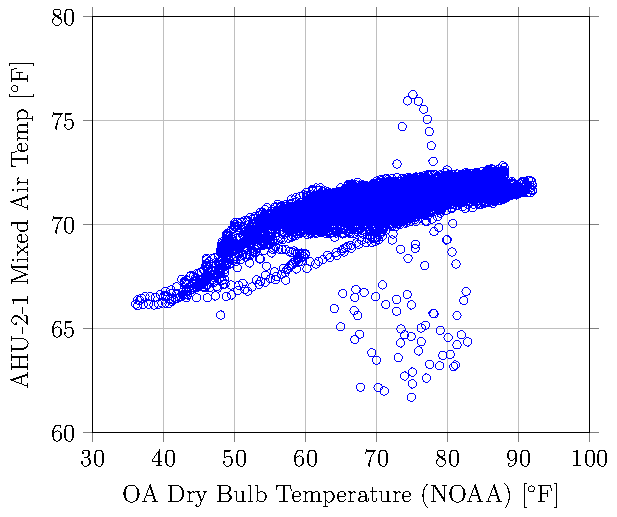
\includegraphics[]{Plots/2016-06-13-1441-AHU21MixedAirTempvsOADryBulbTemperatureNOAA.pdf}
\caption{AHU-2-1 mixed air temperature vs. outdoor air temperature.}
\label{fig:AHU21MixedAirTempvsOADryBulbTemperatureNOAA}
\end{figure}


\begin{figure}
\centering
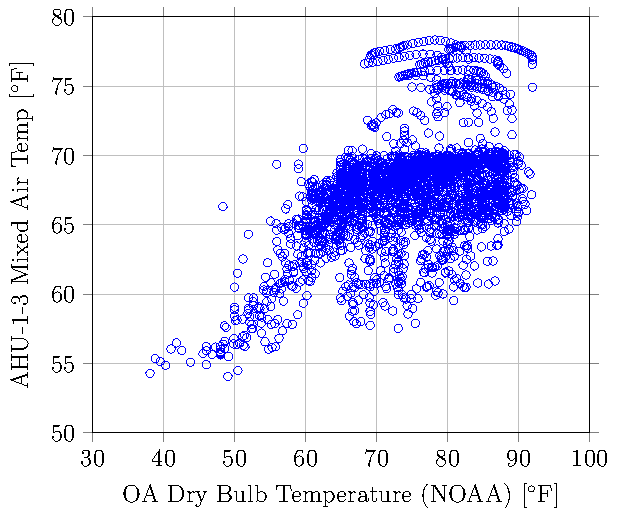
\includegraphics[]{Plots/2016-06-13-1459-AHU13MixedAirTempvsOADryBulbTemperatureNOAA.pdf}
\caption{AHU-1-3 mixed air temperature vs. outdoor air temperature.}
\label{fig:AHU13MixedAirTempvsOADryBulbTemperatureNOAA}
\end{figure}


The result of a \textit{nearest neighbor} approach is shown in \figref{} \ref{fig:AHU13MixedAirTempvsOADryBulbTemperatureNOAA-2}. The algorithm looked back in history (at least a day before) under the following parameters:

\begin{itemize}
    \item The same day of the week
    \item Same hour of day \(\pm\)1 hr.
    \item Same \(\oat{}\) \(\pm\)3\(^\circ\)F
    \item Searching backwards incrementally until 30 data points found
\end{itemize}

The median of the found data points is the resulting prediction. The following plots show the model fits for the different air handling units at NCTM. The data covers a period of 180 days. Figures \ref{fig:2016-09-07-1218-AHU12MixedAirTempvsOADryBulbTemperatureNOAA} and \ref{fig:AHU13MixedAirTempvsOADryBulbTemperatureNOAA-2} show that the prediction algorithm can adequately handle the differences from when the air handling unit is on as well as off. The significant amount of spread in the mixed air temperature is due to data in which the air handler turns off and is allowed to drift, typically to higher temperature in the climate of College Station. 

Figures \ref{fig:2016-09-07-1335-MixedAirTempPredictionforContainerAHU12vsAHU12MixedAirTemp} through \ref{fig:2016-09-07-1623-MixedAirTempPredictionforContainerAHU23vsAHU23MixedAirTemp} show the model fits during times when the air handling units are off, ignoring weekends and holidays, and times between 6:00 PM and 8:00 AM.

\newcommand{\matcaption}[1]{#1 mixed air temperature prediction for data from Mar. 10, 2016 - Sept. 5, 2016, not ignoring any data.}

\begin{figure}
\centering
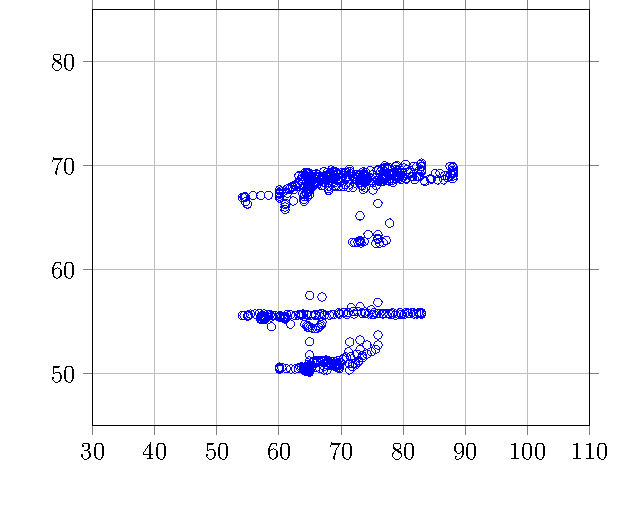
\includegraphics[]{Plots/2016-09-07-1218-AHU12MixedAirTempvsOADryBulbTemperatureNOAA.pdf}
\caption{\matcaption{AHU-1-2}}
\label{fig:2016-09-07-1218-AHU12MixedAirTempvsOADryBulbTemperatureNOAA}
\end{figure}

\begin{figure}
\centering
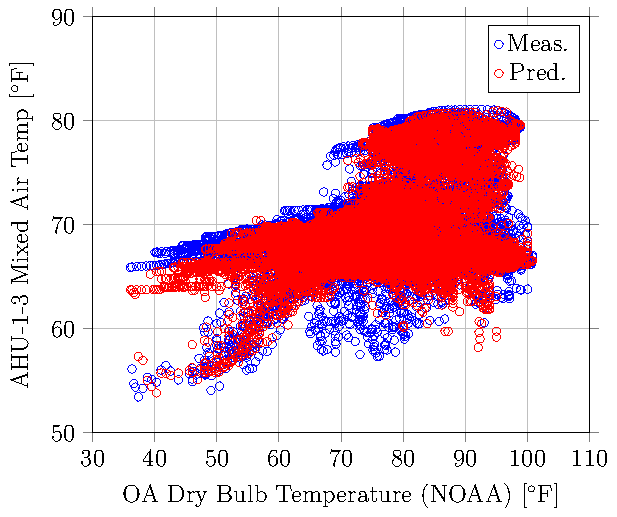
\includegraphics[]{Plots/2016-09-07-0943-AHU13MixedAirTempvsOADryBulbTemperatureNOAA.pdf}
\caption{AHU-1-3 mixed air temperature prediction for data from Mar. 10, 2016 - Sept. 5, 2016, not ignoring any data.}
\label{fig:AHU13MixedAirTempvsOADryBulbTemperatureNOAA-2}
\end{figure}



%% 45 degree plots showing the adequacy of the model fit. 

\begin{figure}
\centering
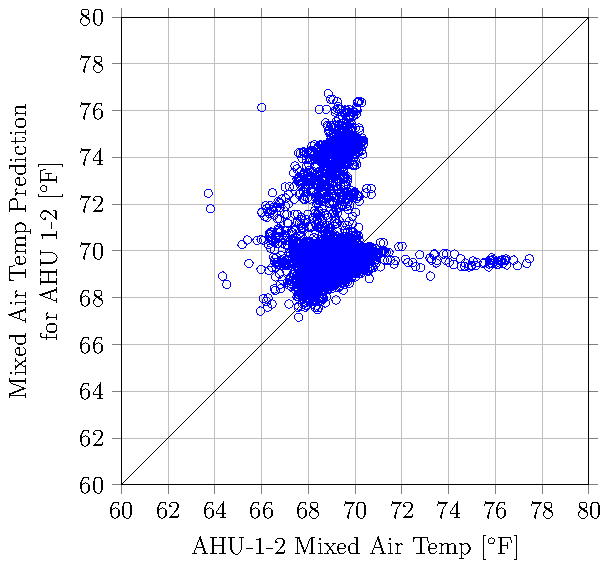
\includegraphics[]{Plots/2016-09-07-1335-MixedAirTempPredictionforContainerAHU12vsAHU12MixedAirTemp.pdf}
\caption{SampleCaption}
\label{fig:2016-09-07-1335-MixedAirTempPredictionforContainerAHU12vsAHU12MixedAirTemp}
\end{figure}

\begin{figure}
\centering
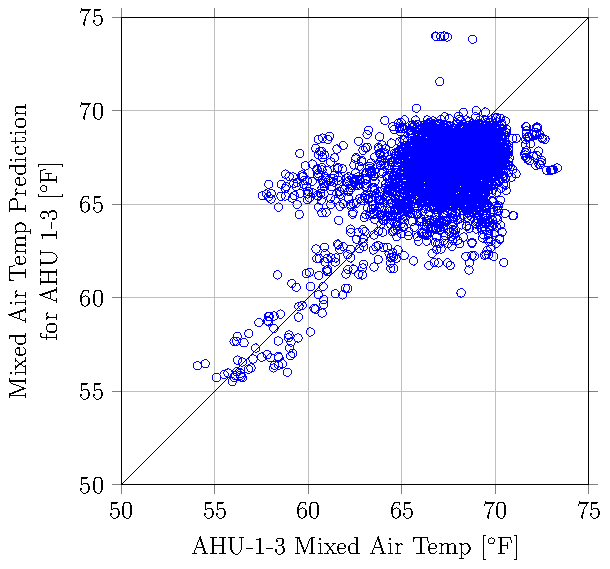
\includegraphics[]{Plots/2016-09-07-1346-MixedAirTempPredictionforContainerAHU13vsAHU13MixedAirTemp.pdf}
\caption{SampleCaption}
\label{fig:2016-09-07-1346-MixedAirTempPredictionforContainerAHU13vsAHU13MixedAirTemp}
\end{figure}

\begin{figure}
\centering
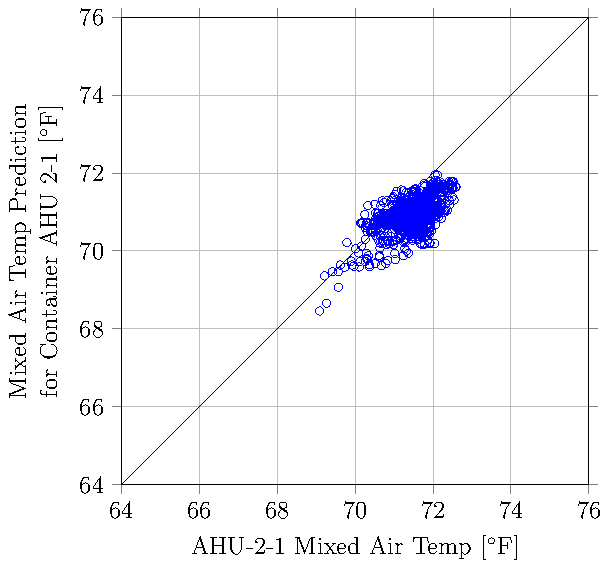
\includegraphics[]{Plots/2016-09-07-1357-MixedAirTempPredictionforContainerAHU21vsAHU21MixedAirTemp.pdf}
\caption{SampleCaption}
\label{fig:2016-09-07-1357-MixedAirTempPredictionforContainerAHU21vsAHU21MixedAirTemp}
\end{figure}

\begin{figure}
\centering
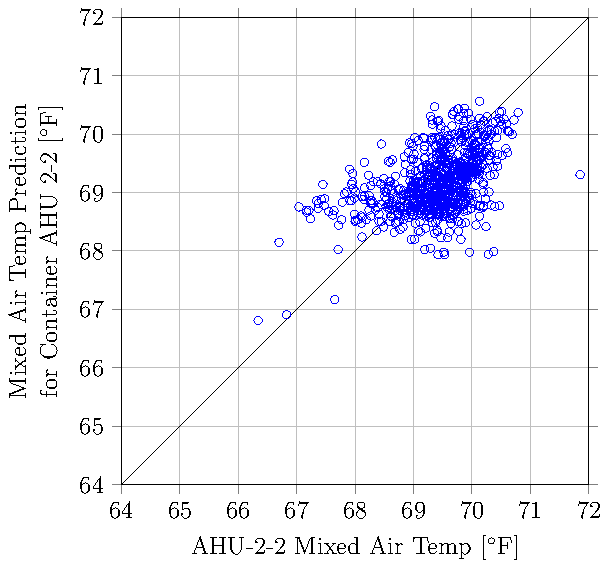
\includegraphics[]{Plots/2016-09-07-1619-MixedAirTempPredictionforContainerAHU22vsAHU22MixedAirTemp.pdf}
\caption{SampleCaption}
\label{fig:2016-09-07-1619-MixedAirTempPredictionforContainerAHU22vsAHU22MixedAirTemp}
\end{figure}

\begin{figure}
\centering
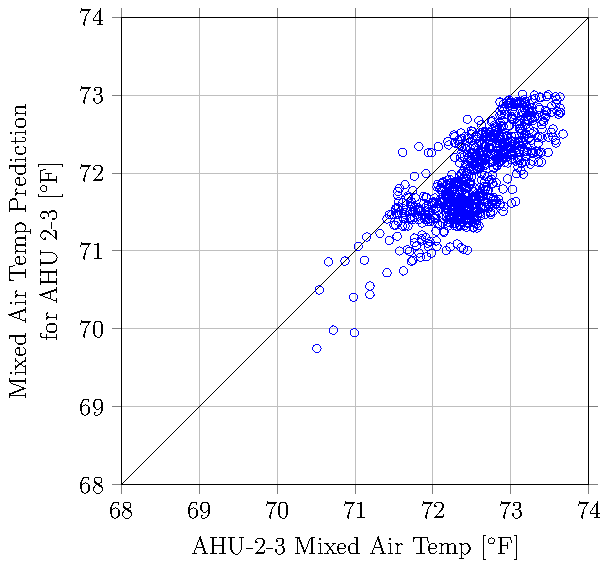
\includegraphics[]{Plots/2016-09-07-1623-MixedAirTempPredictionforContainerAHU23vsAHU23MixedAirTemp.pdf}
\caption{SampleCaption}
\label{fig:2016-09-07-1623-MixedAirTempPredictionforContainerAHU23vsAHU23MixedAirTemp}
\end{figure}


\section{Analysis of the Plenum Air Temperature}

Under certain assumptions, the plenum air temperature for the series fan powered boxes is possible. If the terminal unit is modeled as a simple mixing problem, the plenum air temperature will be 

\begin{equation}
    T_{plenum}=\frac{\flow{tot}T_{dis}-\flow{pri}T_{sa}}{\flow{tot} -\flow{pri}}
\end{equation}

Since \(T_{plenum}\) is a function of 4 variables, it is important to consider the uncertainty in the estimation. Clearly, when \(\flow{plenum}\) is low, assumed to be equivalent to \(\flow{tot} - \flow{pri}\), the uncertainty in  \(T_{plenum}\) grows significantly and when the flow is equal to zero \(T_{plenum}\) is undefined. 

Using the Kline-McKlintock formulation of uncertainty, the uncertainty of \(T_{plenum}\) is 

\begin{multline}
    \delta T_{plen} = \left[\left( \pdv{T_{plen}}{\flow{pri}} \delta \flow{pri}   \right)^2  +\left( \pdv{T_{plen}}{\flow{tot}} \delta \flow{tot}   \right)^2 + \right. \\
    \left. \left( \pdv{T_{plen}}{T_{dis}} \delta T_{dis}   \right)^2 + \left( \pdv{T_{plen}}{T_{sa}} \delta T_{sa}   \right)^2  \right]^{1/2}
\end{multline}

\begin{multline}\label{eq:plenumUncertainty}
    \delta T_{plen} = \left[\left(  \frac{\flow{tot}\left(T_{dis}-T_{sa} \right)}{{\flow{plen}}^2}   \delta \flow{pri} \right)^2  +\left(\frac{\flow{pri}\left(T_{sa}-T_{dis} \right)}{{\flow{plen}}^2}      \delta \flow{tot}   \right)^2 + \right. \\
    \left. \left( \frac{\flow{tot}}{\flow{plen}} \delta T_{dis}   \right)^2 + \left(\frac{\flow{pri}}{\flow{plen}}  \delta T_{sa}   \right)^2  \right]^{1/2}
\end{multline}

So for an example if, 

\newcommand{\flowtotvalue}{\SI{2200}{\CFM}}
\newcommand{\plenflowvalue}{\SI{1000}{\CFM}}

\begin{itemize}
    \item \(\totflow{}=\flowtotvalue\)
    \item \(\plenflow{}=\plenflowvalue\)
    \item \(\priflow=\flowtotvalue - \plenflowvalue = \SI{1200}{\CFM} \)
    \item \(\sat = 55^{\circ}\text{F} \)
    \item \(\dat = 75^{\circ}\text{F} \)
    \item \(\delta\priflow{}=\delta\plenflow=\delta\totflow=100 \text{ CFM}\)
    \item \(\delta \sat = \delta \dat = 1^{\circ} \text{F} \)
\end{itemize}

Equation \ref{eq:plenumUncertainty} becomes
\begin{equation}\label{eq:plenumUncertainty}
    \delta T_{plen} = \left[\left(  \SI{3.06}{\degreeF}  \right)^2  +\left( \SI{-1.39}{\degreeF}  \right)^2 +  \left( \SI{1.83}{\degreeF} \right)^2 + \left(\SI{0.83}{\degreeF}  \right)^2  \right]^{1/2}
\end{equation}

which results in a final uncertainty of \SI{3.91}{\degreeF}.

As an example as to how unstable the calculation for the plenum temperature is, \figref{} \ref{fig:2016-09-16-1006-PlenumTemperatureforContainerFPVAV19vsZoneLoadforContainerFPVAV19} shows the calculation for FPVAV-1-9 over the period from February 1, 2016 - May 1, 2016. The calculated values are unrealistic ranging from -1,500\(^\circ\)F to 1,500\(^\circ\)F. The reason for this is made clear in a time series plots of the flows related to the terminal unit. As shown in \figref{} \ref{fig:2016-09-16-1639-FPVAV19AIRVOLUME-TikzData}, for this particular terminal unit, the primary flow is either near zero or near design. At times, the measured flow is also above the design spec, making the plenum flow calculation zero. When the plenum flow is calculated to be zero, the plenum temperature calculation becomes undefined.


Using the assumptions that the uncertainty in the flow was 100 CFM and the uncertainty in the temperature measurements was 1\(^\circ\)F, the plenum temperature was recorded and plotted versus \(\oat\) from October 6, 2015 to September 12, 2016, ignoring items that appear in \tableref{} \ref{tab:PlenumTemperatureEstimation}. The distribution statistics for each terminal unit is found in \tableref{} \ref{tab:plenumStatistics}. The table is listed in ascending order by the median of the plenum temperature calculated.

To notice is that percentage of ignored points is below 96\% for only 4 terminal units. The majority of the points are ignored because the uncertainy in the calculation is above the 2\(^\circ\)F threshold that was arbitrarily chosen. In fact, at no point was the uncertainy below 2\(^\circ\)F for FPVAV-2-7. The median plenum temperature ranges from 58.8\(^\circ\)F for FPVAV-1-8 to 75.6\(^\circ\)F for FPVAV-1-6.


\begin{table}[]
\centering
\caption{Implementer settings for plenum temperature estimation for NCTM, used to calculate data in \tableref{} \ref{tab:plenumStatistics}.}
\label{tab:PlenumTemperatureEstimation}
\begin{tabular}{@{}rl@{}}
\toprule
Project:         & Mitch Dissertation NCTM---2016-09-19 10:34           \\ \midrule
Scope:           & NCTM                                                 \\
Axis Parameters: & Plenum Temperature vs. OA Drybulb Temp (NOAA)        \\
Date Period:     & 10/6/2015 - 9/12/2016  (342 days)                    \\
OAT range:       & 31 to 100\(^\circ\)F      \\
Ignoring:        & When AHU is Off                                      \\
                 & First 1.0 hours of operation                         \\
                 & Last 1.0 hours of operation                          \\
                 & Sundays                                              \\
                 & Saturdays                                            \\
                 & Federal Holidays                                     \\
                 & Hours from 17:00 to 9:00                             \\
                 & When label Plenum Temp Uncertainty is greater than 2 \\
                 & When label Valve Positions is greater than 1         \\ \bottomrule
\end{tabular}
\end{table}



\begin{figure}
\centering

\includegraphics[]{Plots/2016-09-16-1006-PlenumTemperatureforContainerFPVAV19vsZoneLoadforContainerFPVAV19.pdf}
\caption{Calculated plenum temperature for FPVAV-1-9.}
\label{fig:2016-09-16-1006-PlenumTemperatureforContainerFPVAV19vsZoneLoadforContainerFPVAV19}
\end{figure}

\begin{figure}
\centering
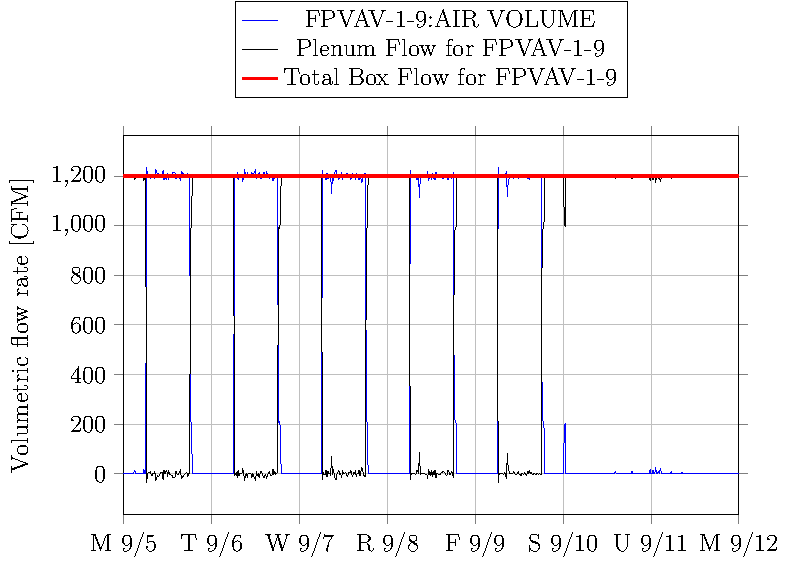
\includegraphics[]{Plots/2016-09-16-1639-FPVAV19AIRVOLUME-TikzData.pdf}
\caption{Flowrates for FPVAV-1-9}
\label{fig:2016-09-16-1639-FPVAV19AIRVOLUME-TikzData}
\end{figure}

\begin{table}[]
\centering
\caption{Calculated plenum temperature statistics for NCTM.}
\label{tab:plenumStatistics}
\begin{tabular}{@{}llllllllll@{}}
    \toprule
    Unit & Min   & \parbox{1cm}{5th \\ Perc.}& Mean  & Median &\parbox{1cm}{95th \\ Perc.} & Max   & \parbox{1cm}{St. \\ Dev. }& \parbox{1cm}{Original\\ Count} & \parbox{1 cm}{\%  \\ Ignored }\\ \midrule
1-8   & 56.5  & 56.5           & 60.6  & 58.8   & 71.8            & 71.8  & 4.25     & 29199          & 99.911\%      \\
2-12 & 52.8  & 55.7           & 60.8  & 61.8   & 62.5            & 75.0  & 2.23     & 29319          & 88.062\%       \\
2-15 & 52.1  & 57.4           & 61.3  & 61.8   & 62.6            & 78.5  & 1.84     & 29324          & 78.645\%       \\
1-9   & 57.0  & 57.0           & 63.6  & 65.0   & 73.5            & 73.8  & 5.34     & 27961          & 99.939\%      \\
2-6   & 65.0  & 65.0           & 65.0  & 65.0   & 65.0            & 65.0  & 0.00     & 29311          & 99.997\%      \\
2-18 & 61.5  & 62.7           & 69.6  & 67.0   & 80.2            & 80.5  & 5.60     & 29312          & 99.846\%      \\
2-16 & 67.0  & 67.0           & 67.3  & 67.5   & 67.5            & 67.5  & 0.29     & 29325          & 99.990\%      \\
2-10 & 66.5  & 66.5           & 67.8  & 67.8   & 69.0            & 69.0  & 1.44     & 29236          & 99.986\%      \\
2-14 & 60.0  & 61.0           & 68.8  & 68.5   & 79.0            & 79.8  & 6.28     & 29318          & 99.860\%      \\
2-11 & 66.5  & 66.5           & 68.0  & 68.5   & 69.5            & 69.5  & 1.01     & 28557          & 99.958\%      \\
2-5   & 68.5  & 68.5           & 69.1  & 69.0   & 70.0            & 70.0  & 0.65     & 29309          & 99.983\%      \\
2-8   & 68.2  & 69.1           & 70.0  & 70.0   & 70.7            & 72.5  & 0.55     & 29304          & 98.601\%       \\
2-13 & 68.0  & 68.5           & 70.0  & 70.0   & 71.5            & 72.6  & 1.34     & 29312          & 99.887\%      \\
1-5   & 55.0  & 63.8           & 71.1  & 70.1   & 78.0            & 79.0  & 4.62     & 30170          & 99.450\%       \\
2-17 & 61.5  & 68.5           & 70.3  & 70.4   & 71.5            & 72.5  & 1.23     & 29287          & 99.126\%       \\
2-2   & 52.5  & 67.3           & 70.7  & 70.8   & 73.6            & 75.6  & 2.69     & 29363          & 98.685\%       \\
1-7   & 60.0  & 64.5           & 71.8  & 71.8   & 75.1            & 75.7  & 3.11     & 29955          & 99.222\%       \\
2-3   & 64.5  & 71.0           & 73.0  & 72.8   & 75.3            & 76.2  & 1.49     & 29367          & 96.391\%       \\
1-2   & 67.0  & 70.8           & 73.9  & 72.9   & 77.8            & 78.5  & 2.60     & 30166          & 99.589\%      \\
2-1   & 67.5  & 70.8           & 73.6  & 73.8   & 75.5            & 81.7  & 1.44     & 29366          & 96.016\%       \\
1-3   & 71.4  & 72.6           & 74.2  & 74.4   & 75.4            & 76.9  & 0.94     & 30145          & 98.202\%       \\
2-9   & 69.0  & 70.7           & 73.9  & 74.5   & 76.5            & 78.4  & 1.88     & 29272          & 76.356\%       \\
1-1   & 57.0  & 71.8           & 74.6  & 74.8   & 79.0            & 82.5  & 2.64     & 30152          & 97.652\%       \\
1-10 & 58.5  & 62.0           & 73.8  & 74.9   & 76.0            & 78.2  & 3.61     & 29941          & 99.008\%       \\
1-4   & 54.0  & 72.4           & 74.9  & 75.1   & 77.2            & 81.7  & 2.51     & 30086          & 98.488\%       \\
2-4   & 69.5  & 73.7           & 75.3  & 75.2   & 76.7            & 77.6  & 0.96     & 29304          & 86.916\%       \\
1-6   & 56.5  & 66.2           & 74.1  & 75.6   & 81.3            & 81.6  & 5.43     & 30170          & 99.738\%      \\
2-7   & N/A & N/A          & N/A & N/A  & N/A           & N/A & N/A    & 28906          & 100.000\%    \\ \bottomrule
\end{tabular}
\end{table}



\section{Analysis of Zone Load Predictions}

An important factor in the optimization methodology is the prediction of the zone loads at a given time, without access to current live sensor information. 

Before analyzing the prediction ability of different zone loads, it is important to gather insight into the nature of the calculated variable that is proposed to be used as the surrogate for zone load.   

If the zone loads are being met and steady-state conditions are assumed, the sensible zone load will be

\begin{equation}
    Q_{zone}=\flow{z} \rhocp{} \left(T_{dis}-T_{z} \right) \approx 1.08 \cdot \flow{z}\left(T_{dis}-T_{z} \right)
\end{equation}

A useful simplification would be replacing the \(\rhocp{}\) term with a constant value. A value of 1.08, when \(\flow{z}\) is in units of CFM and temperature is in units of \(^\circ\)F is common, and is used from this point forward in the estimation of the zone load.

As a result of the dynamics of how  terminal units are actually controlled, the estimated zone load can vary back and forth, while the true zone load is a more smooth function. \figref{} \ref{fig:2016-06-22-1654-ZoneLoadforContainerFPVAV17-TikzData} shows how the estimated zone load can change directionality several times over the course of a day. The zone load for terminal unit FPVAV-1-7 typically varied from 6,000 BTU/hr to 20,000 BTU/hr over the course of the week from June 6, 2016 to June 11, 2016.

\figref{} \ref{fig:2016-06-22-1643-ZoneLoadforContainerFPVAV22-TikzData} shows another example of how the estimated zone load may vary throughout a typical week. \figref{} \ref{fig:2016-06-22-1643-ZoneLoadforContainerFPVAV22-TikzData} shows the zone load for FPVAV-2-2, which experiences a significant load compared to the other terminal units at NCTM. the zone load varies from near 10,000 BTU/hr to near 50,000 BTU/hr at its peak.

With \figref{} \ref{fig:2016-06-22-1654-ZoneLoadforContainerFPVAV17-TikzData} as evidence, it is clear that the ``true'' zone load cannot be reasonably estimated with the trend data that is available in typical BAS systems. However, the ratio of magnitudes of the load from zone to zone can still be inferred and be useful in improving the energy efficiency of the system.  

\begin{figure}
\centering
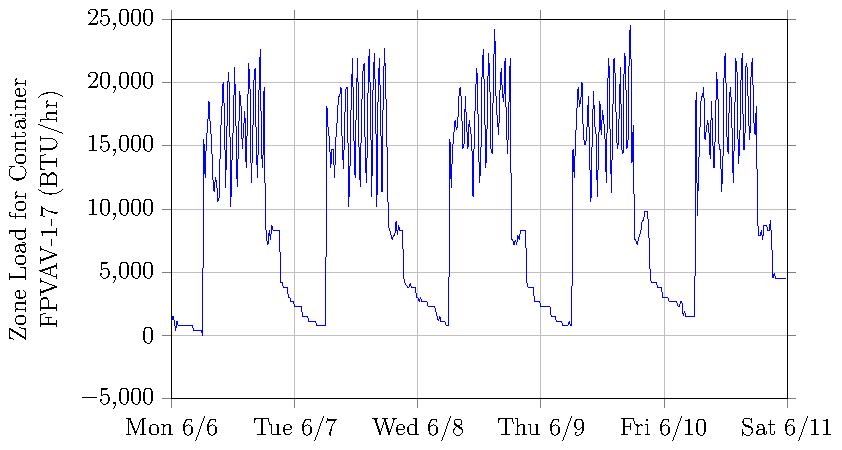
\includegraphics[]{Plots/2016-06-22-1654-ZoneLoadforContainerFPVAV17-TikzData.pdf}
\caption{Zone load estimation for FPVAV-1-7.}
\label{fig:2016-06-22-1654-ZoneLoadforContainerFPVAV17-TikzData}
\end{figure}

\begin{figure}
\centering
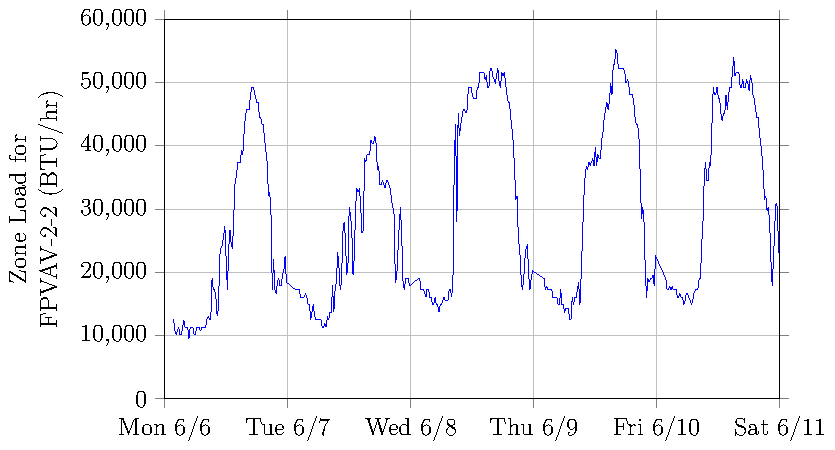
\includegraphics[]{Plots/2016-06-22-1643-ZoneLoadforContainerFPVAV22-TikzData.pdf}
\caption{Zone load estimation for FPVAV-2-2.}
\label{fig:2016-06-22-1643-ZoneLoadforContainerFPVAV22-TikzData}
\end{figure}



\figref{} \ref{fig:ZoneLoadforContainerFPVAV214vsOADryBulbTemperatureNOAA} shows an example of the zone load plotted against outdoor air dry-bulb temperature. Notice that the load is not a well defined function of \(\oat\). This turns out to be the case for many of the internal zones, which will be related more to the time of day parameters. 

\figref{} \ref{fig:ZoneLoadforContainerFPVAV29vsOADryBulbTemperatureNOAA} shows the zone load for FPVAV-2-9 versus \(\oat\). FPVAV-2-9 serves only internal zones, and the load only ranges from approximately 250 BTU/hr to 4,000 BTU/hr.


\begin{figure}
\centering
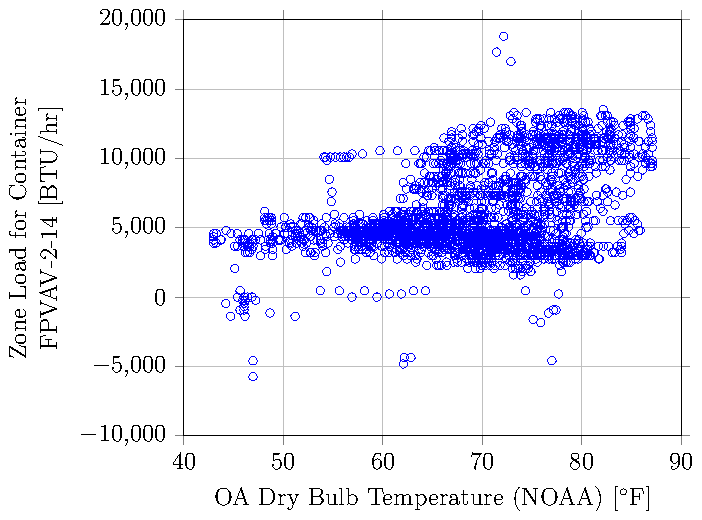
\includegraphics[]{Plots/2016-06-22-1704-ZoneLoadforContainerFPVAV214vsOADryBulbTemperatureNOAA.pdf}
\caption{Calculated zone load for FPVAV-2-14 during the month of April 2016.}
\label{fig:ZoneLoadforContainerFPVAV214vsOADryBulbTemperatureNOAA}
\end{figure}


\begin{figure}
\centering
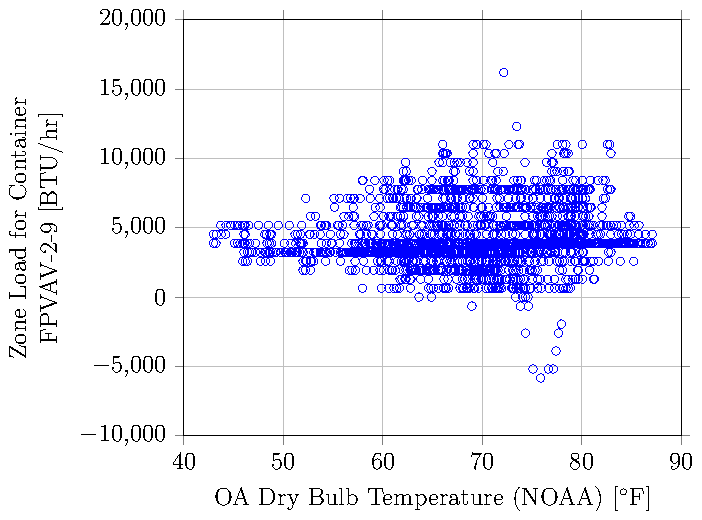
\includegraphics[]{Plots/2016-06-22-1716-ZoneLoadforContainerFPVAV29vsOADryBulbTemperatureNOAA.pdf}
\caption{Calculated zone load for FPVAV-2-9, which serves only internal space, during the month of April 2016.}
\label{fig:ZoneLoadforContainerFPVAV29vsOADryBulbTemperatureNOAA}
\end{figure}


The statistics related to the predictions of the zone loads for data ranging from October 6, 2015 to June 1, 2016 is given in \tableref{} \ref{tab:zoneLoadStats}.


%%Data from NCTM Report 2016-06-20 T 12-16.xlsx.
\begin{table}[]
\centering
\caption{Statistics related to the prediction of the zone loads at NCTM.}
\small
\label{tab:zoneLoadStats}
\begin{tabular}{lrrrr} 
    \toprule
    Terminal Unit & \parbox{2.3cm}{Med. Abs. \\ \(\epsilon\) (BTU/hr)}  & \parbox{2.3cm}{Mean Abs.\\\(\epsilon\)  (BTU/hr)} & \parbox{2cm}{RMSE \\ (BTU/hr)} & \parbox{2cm}{MBE \\ (BTU/hr)}\\
    \midrule
FPVAV-2-7 & 108 & 171 & 298 & -41 \\ 
FPVAV-2-16 & 135 & 385 & 704 & 59 \\ 
FPVAV-2-5 & 162 & 221 & 328 & -22 \\ 
FPVAV-2-12 & 203 & 1,058 & 1,885 & -896 \\ 
FPVAV-2-6 & 216 & 488 & 836 & 24 \\ 
FPVAV-2-13 & 270 & 784 & 1,841 & 68 \\ 
FPVAV-2-10 & 292 & 631 & 1,000 & -87 \\ 
FPVAV-2-11 & 302 & 708 & 1,062 & -68 \\ 
FPVAV-2-18 & 324 & 914 & 1,614 & 77 \\ 
FPVAV-1-11 & 324 & 703 & 1,585 & 115 \\ 
FPVAV-2-14 & 459 & 1,004 & 1,780 & -9 \\ 
FPVAV-2-4 & 540 & 1,036 & 2,012 & 84 \\ 
FPVAV-1-2 & 626 & 1,201 & 2,056 & -385 \\ 
FPVAV-2-8 & 648 & 991 & 1,519 & -43 \\ 
FPVAV-2-9 & 648 & 1,236 & 1,763 & 635 \\ 
FPVAV-2-17 & 691 & 1,386 & 2,327 & 122 \\ 
FPVAV-2-15 & 756 & 3,852 & 12,353 & 552 \\ 
FPVAV-1-8 & 945 & 1,371 & 1,978 & 336 \\ 
FPVAV-2-3 & 972 & 1,789 & 3,587 & -171 \\ 
FPVAV-2-1 & 1,080 & 1,609 & 2,871 & -559 \\ 
FPVAV-1-9 & 1,296 & 1,850 & 2,805 & 209 \\ 
FPVAV-1-5 & 1,404 & 2,463 & 4,105 & -17 \\ 
FPVAV-1-10 & 1,512 & 2,819 & 4,634 & 1,054 \\ 
FPVAV-1-1 & 1,598 & 3,783 & 6,267 & -1,359 \\ 
FPVAV-1-3 & 1,755 & 3,164 & 4,868 & -237 \\ 
FPVAV-1-6 & 1,814 & 3,186 & 4,861 & 261 \\ 
FPVAV-1-7 & 2,268 & 2,827 & 3,942 & -326 \\ 
FPVAV-2-2 & 2,376 & 4,422 & 7,184 & 1,773 \\ 
FPVAV-1-4 & 3,024 & 5,569 & 8,502 & 19 \\ 
    \bottomrule
\end{tabular}
\end{table}

The highest errors in the prediction were for FPVAV-1-4, the zone that has the highest overall zone load in the building, by a significant margin. It has estimated loads near 50,000 BTU/hr.


%% These items come from the analysis done with plus minus 15 min and 3 degree F OAT bounds in file Batch Plots -- Mitch Dissertation N -- 2016-09-14 0952

An interesting pattern that was that the initial prediction routine overpredicted the zone load when the zone load was closer to the heating range and underpredicted the zone load during times of high cooling load. This bias was seen in every terminal unit in the building and this bias occured with both the largest and smallest terminal units. Figures \ref{fig:2016-09-14-1028-ZoneLoadResidualforContainerFPVAV22vsZoneLoadforContainerFPVAV22} through \ref{fig:2016-09-14-1020-ZoneLoadResidualforContainerFPVAV27vsZoneLoadforContainerFPVAV27} show examples of this phenomenon. The date period analyzed was from March 1, 2016 to August 1, 2016, ignoring when the AHUs were off, federal holidays and weekends, and hours from 5 PM to 9 AM. 

\newcommand{\zoneLoadCaption}[1]{Bias in zone load prediction for #1.}

\begin{figure}
\centering
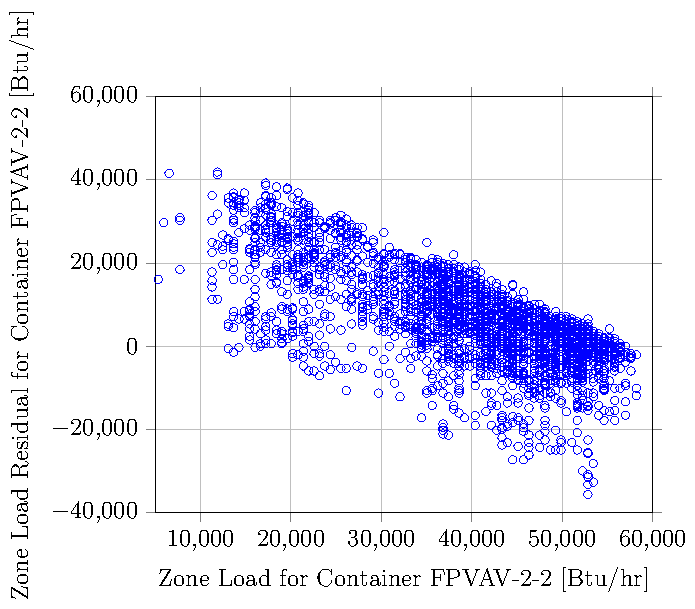
\includegraphics[]{Plots/2016-09-14-1028-ZoneLoadResidualforContainerFPVAV22vsZoneLoadforContainerFPVAV22.pdf}
\caption{\zoneLoadCaption{FPVAV-2-2}}
\label{fig:2016-09-14-1028-ZoneLoadResidualforContainerFPVAV22vsZoneLoadforContainerFPVAV22}
\end{figure}

\begin{figure}
\centering
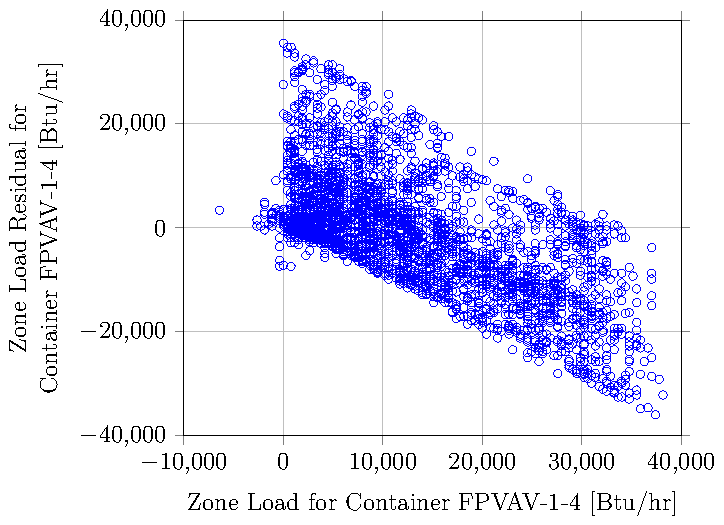
\includegraphics[]{Plots/2016-09-14-1007-ZoneLoadResidualforContainerFPVAV14vsZoneLoadforContainerFPVAV14.pdf}
\caption{\zoneLoadCaption{FPVAV-1-4}}
\label{fig:2016-09-14-1007-ZoneLoadResidualforContainerFPVAV14vsZoneLoadforContainerFPVAV14}
\end{figure}

\begin{figure}
\centering
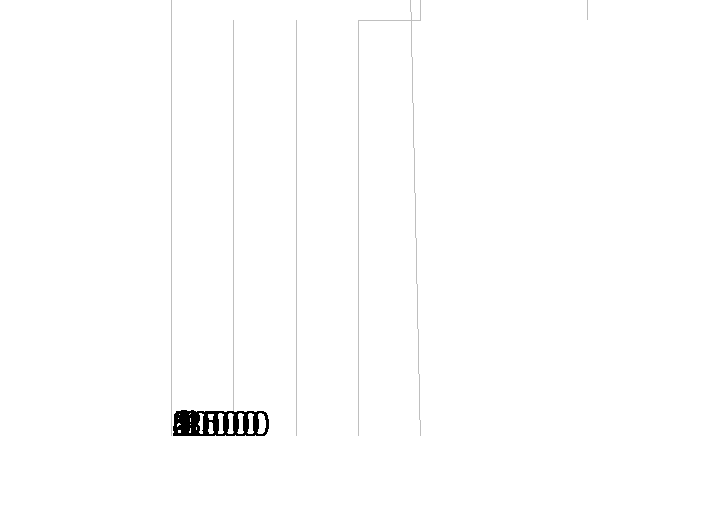
\includegraphics[]{Plots/2016-09-14-1020-ZoneLoadResidualforContainerFPVAV27vsZoneLoadforContainerFPVAV27.pdf}
\caption{ \zoneLoadCaption{FPVAV-2-7} }
\label{fig:2016-09-14-1020-ZoneLoadResidualforContainerFPVAV27vsZoneLoadforContainerFPVAV27}
\end{figure}


\section{Analysis of the Mixed Air Temperature in Series Terminal Unit and Reheat Assumption}

For series fan powered boxes, the assumption was made that the total flow remains constant and that the mixed air temperature at the individual box can be predicted based on the primary flow value that is measured. 


\section{Analysis of the Critical Zone Assumption}

The critical zone/damper is to be used to determine the static pressure setpoint that can be used to supply the desired flows found from the optimization. An important consideration in the methodology is checking how how this assumption holds. Data from NCTM can be used to test the validity of the approach.

The following figures show the maximum damper position of the children terminal units for each of the air handlers during the month of April 2016. During this time, for AHU-2-1 and AHU-2-2, there was no time in which a terminal unit damper was fully open which indicates that there is potential for the supply air static pressure setpoint to be reduced.  

\newcommand{\MaxDampCaption}[1]{Maximum damper position of all children terminal units versus \(\oat{}\) for #1 during the month of April 2016.}

\begin{figure}
\centering
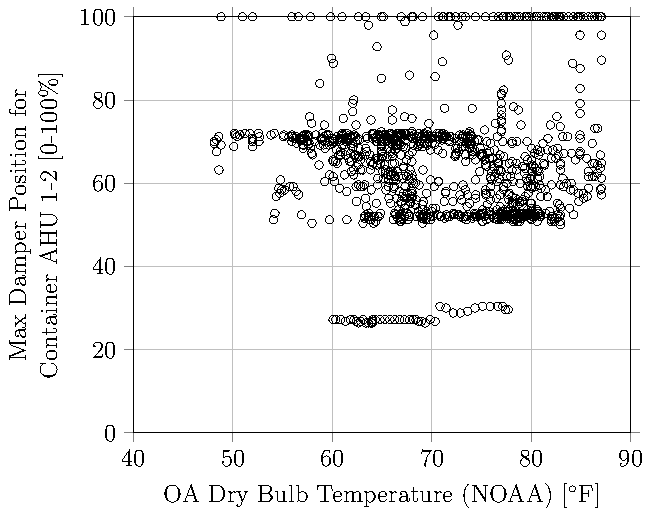
\includegraphics{Plots/MaximumDamperPosition-1-2.pdf} 
\caption{\MaxDampCaption{AHU-1-2}}
\label{fig:MaxDamperPositionforContainerAHU12vsOADryBulbTemperatureNOAA}
\end{figure}

\begin{figure}
\centering
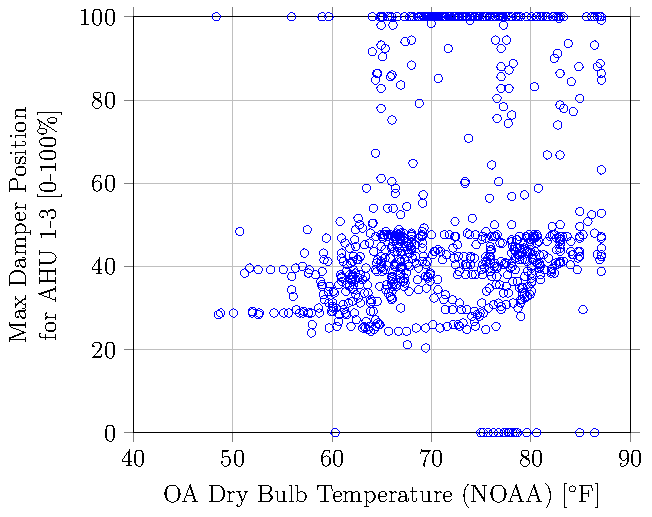
\includegraphics{Plots/MaximumDamperPosition-1-3.pdf}
\caption{\MaxDampCaption{AHU-1-3}}
\label{fig:MaxDamperPositionforContainerAHU13vsOADryBulbTemperatureNOAA}
\end{figure}


\begin{figure}
\centering
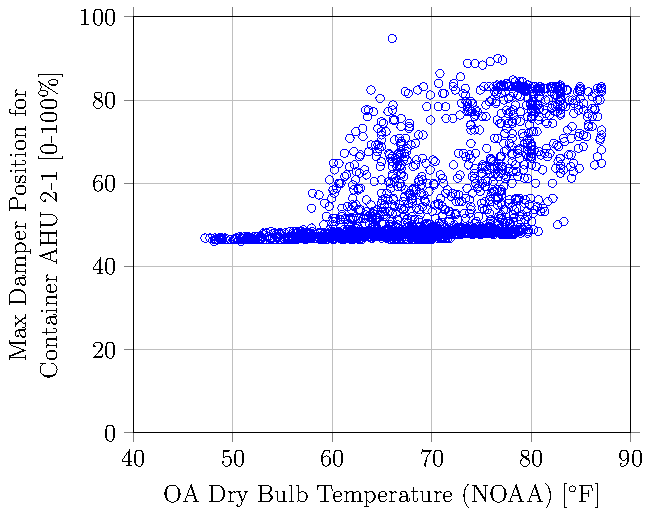
\includegraphics{Plots/MaximumDamperPosition-2-1.pdf}
\caption{\MaxDampCaption{AHU-2-1}}
\label{fig:MaxDamperPositionforContainerAHU21vsOADryBulbTemperatureNOAA}
\end{figure}

\begin{figure}
\centering
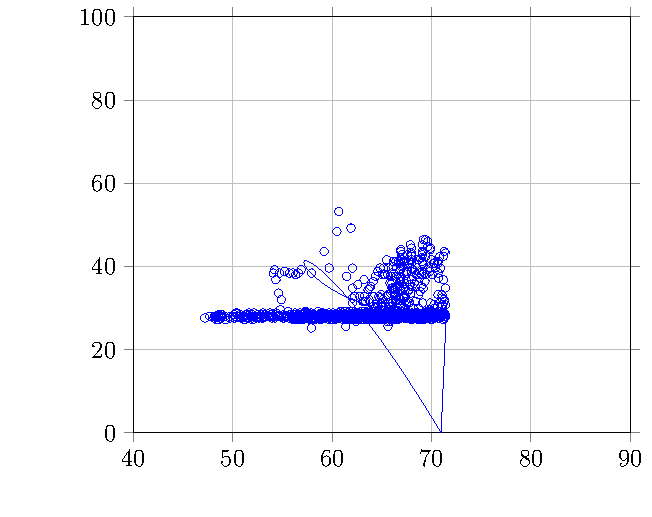
\includegraphics{Plots/2016-06-06-1427-MaxDamperPositionforContainerAHU22vsOADryBulbTemperatureNOAA.pdf}
\caption{\MaxDampCaption{AHU-2-2}}
\label{fig:MaxDamperPositionforContainerAHU22vsOADryBulbTemperatureNOAA}
\end{figure}

\begin{figure}
\centering
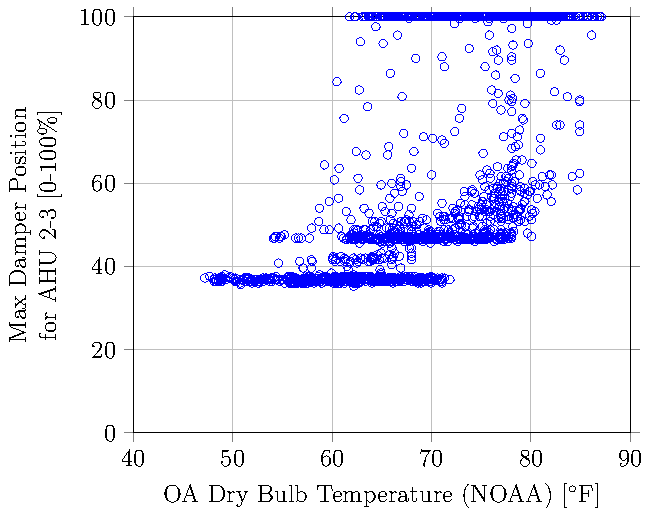
\includegraphics[]{Plots/2016-06-06-1454-MaxDamperPositionforContainerAHU23vsOADryBulbTemperatureNOAA.pdf}
\caption{\MaxDampCaption{AHU-2-3}}
\label{fig:MaxDamperPositionforContainerAHU23vsOADryBulbTemperatureNOAA}
\end{figure}


\subsection{Critical Zones for NCTM}

An investigation into the critical zones based on historical data was completed. 15 minute interval data from Jan. 1, 2016 through Jun. 1, 2016 was used to check which damper positions were most open at a given timestamp. \tableref{} \ref{tab:AHU12CriticalZone} shows the results of this analysis. In all five of the applicable air handling units, there is a damper that is critical at least 59\% of the time. 

%% Comes from file 2016-06-08-1603-CriticalZoneAnalysis.xlsx
%% Run from 2016-01-01 to 2016-06-01.
%% Assumes that the AHU is on. 
\begin{table}
\centering
\caption{Percentage of time that different boxes for various AHUs were the most open during the period of Jan. 1, 2016 - Jun. 1, 2016.}
\label{tab:AHU12CriticalZone}
\begin{tabular}{@{}llll@{}}
\toprule
AHU                       &  Tbox       & Count of Max & Percent as Critical \\ \midrule
\multirow{3}{*}{AHU-1-2}  &  FPVAV-1-8  & 3,518        & 68\%                \\
                          &  FPVAV-1-9  & 1,281        & 25\%                \\
                          &  2 others   & 354          & 7\%                 \\ \midrule
\multirow{3}{*}{AHU-1-3} & FPVAV-1-5 & 2,331        & 59\%                \\
                         & FPVAV-1-4 & 1,006        & 25\%                \\
                         & 4 others  & 622          & 15\%                 \\ \midrule
\multirow{3}{*}{AHU-2-1} &  FPVAV-2-1   &   10,965   &    79\%  \\
                         &  FPVAV-2-2   &   2,648   &    19\%  \\
                         &  FPVAV-2-3   &   258   &    2\% \\ \midrule
\multirow{3}{*}{AHU-2-2} &    FPVAV-2-18   &   	10,003	&  72\%  \\
&  FPVAV-2-14   &    	3,171   &  	23\%  \\
&  6 others   &   	648	&  5\%  \\ \midrule
\multirow{3}{*}{AHU-2-3}  & FPVAV-2-6   &   9,883     &   72\%  \\ 
                        & FPVAV-2-11     &   3,743     &   27\%  \\ 
                        & FPVAV-2-10     &   184     &   1\%  \\ \midrule
\end{tabular}
\end{table}


\subsection{Accuracy of Mechanical Specifications}

In simplified analysis and modeling such as being proposed, it would be ideal if the specifications in the mechanical drawings can be used directly. One important parameter is the design flow rate for the terminal unit. \tableref \ref{tab:TerminalUnitInformation} shows the design flow rates for all the series fan powered terminal units in the NCTM building. The results show that the design specifications were sufficiently accurate.  All data that were available at the time (October 6, 2015 through June 7, 2016) were analyzed to capture a large number of timestamps (over 22,000 timestamps). There are several reasons for potential differences between the maximum measured flow and the design flow rates in the mechanical drawings. It may be the case that the terminal unit was oversized and the design flow rate was never neccessary. There may be bias in the flow rate measurements.  

The largest percent difference and absolute difference between the measured maximum flow rate and design value was for FPVAV-1-9. The difference was due to less than 15 outliers in the data (out of over 20,000 data points in total), and if they were to be removed, the maximum is in line with the design value of 1,200 CFM for the vast majority of the data, as seen in \figref{} \ref{fig:FPVAV19AIRVOLUMEvsFPVAV19DMPRCOMD}. 

%%See file: Batch Plots -- Mitch Dissertation N -- 2016-06-09 0942.xlsx
\begin{table}[]
\centering
\footnotesize
\caption{Comparison of design flow specifications to actual data.}
\label{tab:TerminalUnitDesignSpecCheck}
\begin{tabular}{@{}llrl@{}}
\toprule
AHU &  Terminal Unit & \parbox{1.5cm}{\centering  Flow\\(CFM)}  & \parbox{2.7cm}{Maximum Meas. \\  Flow (CFM)}  \\ \midrule
%%\parbox{2cm}{AHU-1-1 \\ (5 hp)} & \multicolumn{3}{l}{No boxes - Serves Teaching Module alone, Constant Fan} \\ \midrule
AHU-1-2        & FPVAV-1-7 & 1,400 & 1,496  \\ \cmidrule(r){2-4}
(5 hp)         & FPVAV-1-8 & 700 &  840     \\  \cmidrule(r){2-4}
               & FPVAV-1-9 & 1,200 &  1,688 \\  \cmidrule(r){2-4}
               & FPVAV-1-10 & 1,600 & 1,712 \\\midrule
AHU-1-3        & FPVAV-1-1 & 1,480 &  1,676 \\  \cmidrule(r){2-4}
(7.5 hp)       & FPVAV-1-2 & 1,160 & 1,240  \\  \cmidrule(r){2-4}
               & FPVAV-1-3 & 1,300 & 1,364  \\  \cmidrule(r){2-4}
               & FPVAV-1-4 & 1,400 & 1,760  \\  \cmidrule(r){2-4}
               & FPVAV-1-5 & 1,040 & 612    \\  \cmidrule(r){2-4}
               & FPVAV-1-6 & 1,120 & 1,288  \\\midrule
%%\parbox{2cm}{AHU-1-4 \\ (7.5 hp)} & \multicolumn{3}{l}{No boxes - Serves open atrium outside lecture halls, constant fan}  \\\midrule
AHU-2-1         & FPVAV-2-1 & 2,000 & 2,016 \\  \cmidrule(r){2-4}
   (7.5 hp)     & FPVAV-2-2 & 2,200 & 2,060 \\  \cmidrule(r){2-4}
                & FPVAV-2-3 & 1,800 & 1,824  \\\midrule
AHU-2-2         & FPVAV-2-9 & 2,400 & 2,448  \\  \cmidrule(r){2-4}
(10 hp)         & FPVAV-2-12 & 500 & 452  \\  \cmidrule(r){2-4}
               & FPVAV-2-13 & 1,000 &  1,032 \\  \cmidrule(r){2-4}
               & FPVAV-2-14 & 850 &  892     \\  \cmidrule(r){2-4}
               & FPVAV-2-15 & 1,400 & 1,332\\  \cmidrule(r){2-4}
               & FPVAV-2-16 & 500 & 484\\  \cmidrule(r){2-4}
               & FPVAV-2-17 & 1,280 & 1,304\\  \cmidrule(r){2-4}
               & FPVAV-2-18 & 600 & 604   \\\midrule
AHU-2-3  & FPVAV-2-4 & 2,000 & 1,944  \\  \cmidrule(r){2-4}
        (7.5 hp)       & FPVAV-2-5 & 600 & 504\\  \cmidrule(r){2-4}
               & FPVAV-2-6 & 400 & 228  \\  \cmidrule(r){2-4}
               & FPVAV-2-7 & 200 & 252 \\  \cmidrule(r){2-4}
               & FPVAV-2-8 & 1,200 & 1,184\\  \cmidrule(r){2-4}
               & FPVAV-2-10 & 540 & 588 \\  \cmidrule(r){2-4}
               & FPVAV-2-11 & 560 & 656  \\ \bottomrule
\end{tabular}
\end{table}

%%See file: Batch Plots -- Mitch Dissertation N -- 2016-06-09 0942.xlsx
\begin{figure}
\centering
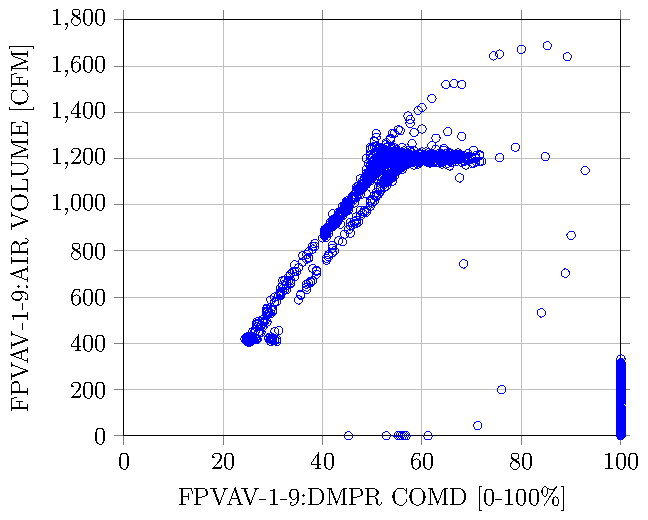
\includegraphics[]{Plots/2016-06-09-1038-FPVAV19AIRVOLUMEvsFPVAV19DMPRCOMD.pdf}
\caption{Damper position versus primary air flow for FPVAV-1-9.}
\label{fig:FPVAV19AIRVOLUMEvsFPVAV19DMPRCOMD}
\end{figure}

\section{Discussion}

Based on the previous results, several conclusions can be gathered that relate to the propsed work.

The first is that it appears plausible that the ``zone load'' can be reasonably estimated to provide useful optimization. In fact, the general relationship in the size of the thermal loads of the different zones is more important than the precise value, of which the data available is not capable of estimating. 

The second is that the design specifications from mechanical drawings can be used as the first approximation for flows and power. There was general agreement between the terminal unit design flows and the actual maximum realized flows at NCTM, as seen in \tableref{} \ref{tab:TerminalUnitDesignSpecCheck}. 
